\documentclass[a4paper,10pt]{report}
\usepackage[utf8]{inputenc}
\usepackage[T1]{fontenc}
\usepackage[french]{babel}
\usepackage{graphicx}
\usepackage{ulem}
\usepackage{float}
\usepackage{amsmath}
\usepackage{amssymb}
\usepackage{mathrsfs}
\usepackage{color}
\usepackage{fancyhdr}
\usepackage{pdfpages}
\usepackage{layout}
\usepackage{multicol}
\usepackage{setspace}
\usepackage{tabularx,array}
\usepackage{tikz, tkz-tab}
\usepackage[top=2cm,bottom=2cm,left=2cm,right=2cm]{geometry}
\usepackage[colorlinks=true]{hyperref}
\usepackage{amsthm}
\usepackage{listings}
\setlength{\parindent}{0cm}
\setlength{\parskip}{1ex plus 0.5ex minus 0.2ex}
\newcommand{\hsp}{\hspace{20pt}}
\newcommand{\HRule}{\rule{\linewidth}{0.1mm}}

\newcolumntype{Y}{>{\centering\arraybackslash}X}
\begin{document}
\begin{spacing}{1.5}
\graphicspath{{image/}}
\begin{titlepage}
\begin{sffamily}
\begin{center}
\vspace*{\stretch{1}}
\textsc{\LARGE Eirbot \\ Coupe de France de robotique}\\[2cm]
\HRule \\[0.4cm]
{\huge \bfseries Equipe Eirboat \\[0.4cm]}

\HRule \\[2cm]

\textsc{\Large 1A 2019-2020}\\[2cm]
              
\includegraphics[scale=0.3]{LogoEirbot.png} \vfill

\vspace*{\stretch{1}}
  \end{center}
  \end{sffamily}
\end{titlepage}

\setcounter{tocdepth}{1}
\tableofcontents
\newpage
\part{Rapports de réunion}
\pagestyle{fancy}
\lhead{Eirboat}
\chead{\textbf{Rapports de réunion}}
\rhead{\thepage}
\lfoot{}
\cfoot{}
\rfoot{}
 \fancyfoot[R]
 {
 
\includegraphics[scale=0.075]{65508.png}
 }

\section*{Jeudi 24 Octobre}
\paragraph*{Ordre du jour.}
\begin{itemize}
\item Définir les différentes tâches que doit remplir le robot
\item Donner une première idée de ce que les gens doivent faire
\end{itemize}
\begin{multicols}{2}
\paragraph*{Tâches à faire par le robot.}
Une version détaillée est disponible en \ref{taches}
\begin{itemize}
\item Se mouvoir (soft)
\item Mécanique générale
\item Détecter les adversaires
\item Détecter les objets
\item Lire la boussole
\item Communiquer
\item Elever le drapeau
\item Actionner les manches à air
\item Alimentation
\item Phare
\end{itemize}
\columnbreak
\paragraph*{Répartition des tâches.}
Une version détaillé est disponible en \ref{repartition}
\begin{itemize}
\item Liam, Emile, Clément, SD
\item Erwann, Valentin, Marion
\item Martin, Liam
\item $\emptyset$
\item Maxime, Emile, Léo
\item SD
\item Filipe, Valentin, Erwann
\item Filipe, Jeremy, Marius
\item Ptit Lu, Yohann, Julien, Léo
\item Marius, Marion
\end{itemize}
\end{multicols}

\paragraph*{Objectifs de la prochaine réunion.}
\begin{itemize}
\item Spécifier les robots
\item Définir précisément les tâches
\item Penser à la stratégie
\end{itemize}

\newpage
\section*{Jeudi 31 Octobre}
Pas de réunion : vacances
\newpage
\section*{Jeudi 7 Octobre}
\paragraph*{Ordre du jour.}
\begin{itemize}
\item Définir les actions à faire
\item Définir une hiérarchie de difficulté dans les actions
\item Définir la mécanique du robot
\end{itemize}

\paragraph*{Définition des méthodes.}
\begin{center}
\begin{tikzpicture}
\tikzstyle{lien}=[->,>=stealth,rounded corners=20pt,thick]
\tikzset{individu/.style={draw,thick,fill=#1!25},
individu/.default={white}}
\node[individu=red] (A) at (0,0 ){\textsc{Détecter adversaire}};
\node[individu] (A1) at (4,1){Système infrarouge};
\node[individu] (A2) at (4,-1 ){\xout{Système LIDAR}};
\draw[lien] (A) -- (A1);
\draw[lien] (A) -- (A2);

\node[individu=red] (B) at (10,0 ){\textsc{Lire Boussole}};
\node[individu] (B1) at (14,1){Balise sur le côté};
\node[individu] (B2) at (14,-1 ){Détecteur sur le robot};
\draw[lien] (B) -- (B1);
\draw[lien] (B) -- (B2);

\node[individu=green] (C) at (0,-5 ){\textsc{Elevation drapeau}};
\node[individu] (C1) at (5,-5){Pignon, cremaillère, ressort};
\draw[lien] (C) -- (C1);

\node[individu=green] (D) at (10,-5 ){\textsc{Manche à air}};
\node[individu] (D1) at (14,-5){Tige qui sort du robot};
\draw[lien]  (D) -- (D1);

\node[individu=orange] (E) at (5,-7 ){\textsc{Phare}};
\node[individu] (E1) at (9,-7){Voir avec Marius};
\draw[lien]  (E) -- (E1);

\node[individu=orange] (F) at (5,-9 ){\textsc{Mécanique générale}};
\node[individu] (F1) at (1,-11){Forme : octognone};
\node[individu] (F2) at (5,-11){Taille : en cours};
\node[individu] (F3) at (9,-11){Motricité : 2 roues + patins};
\draw[lien]  (F) -- (F1);
\draw[lien]  (F) -- (F2);
\draw[lien]  (F) -- (F3);
\end{tikzpicture}
\end{center}

\paragraph*{Description du robot.}
Pour l'instant il se dessine selon 5 étages
\begin{enumerate}
	\item Switch pour le côté de jeu, diode de vérification, porte balise, ON/OFF, Boutons d'arrêt d'urgence.
	\item Porte pavillon, rasp
	\item Porte pavillon, carte numérique
	\item Détecteur IR, carte puissance, actionner manche à air, détecteur IR
	\item moteur, batterie, moteur
\end{enumerate}

\paragraph*{Objectif de la prochaine réunion.}
\begin{itemize}
	\item Avancement table
	\item Avancement méca
	\item Lancer le phare
	\item Lancer l'asservissement
\end{itemize}

\newpage
\section*{Jeudi 14 Novembre}
\paragraph*{Point mécanique.}
Erwann à produit un prototype du robot, il n'est pas complet mais nous donne une idée de ce que nous allons faire. La création du robot est donc en cours.
Pour les premiers test, nous pouvons utiliser la base métallique.

\paragraph*{Point phare.}
La mécanique du phare est au point, il faut rajouter un module de musique, l'actionneur sera identique à celui des manches à air.
Sur le planning le phare pourrait être construit d'ici la prochaine réunion.

\paragraph*{Point asservissement.}
Liam, Emile et Clément commencent à travailler dessus. Ils se sont familiarisés avec les encodeurs et chapterent sur la nucléo.\\
Un résumé de la formation de Mathieu sur l'odométrie : \\
On définit $v_L$ , $v_R$ comme la vitesse gauche et la vitesse droite.
\begin{itemize}
  \item $\text{short} \; v = (\text{short} \; v_{old} - \text{short} \; v_{new})$ %v doit posséder un type de la même dimension que old et new, old et new doivent être du même type
  \item Soit $d$ la distance infinitésimal $$d = \dfrac{v_L+v_R}{2}$$ Soit $\alpha$ l'angle infinitésimal $$\alpha = \dfrac{v_L-v_R}{2}$$
  \item Rafraichissement de la position du robot. \\ Soit $x,y,\theta$ les coordonnées du robot. \begin{enumerate}
  \item $\theta = \theta + \dfrac{\alpha}{2}$
  \item $\begin{cases} x = x + cos(\dfrac{\alpha}{\text{TICKS}}) \times d \\ y = y + sin(\dfrac{\alpha}{\text{TICKS}}) \times d \end{cases}$
  \item $\theta = \theta + \dfrac{\alpha}{2}$
  \item $\text{if}(\text{aps}(\theta) > \pi.\text{TICKS PER RAD})$ \\ $a=a-\text{sg}(a)\times 2 \pi \times \text{TICKS}$
  \end{enumerate}
\end{itemize}
Toutes les codes et les explications sont disponibles sur le github : \url{https://github.com/eirbot/eirbot2019-2A/tree/master/soft/include}

\newpage
\section*{Jeudi 21 Novembre}
Open perdu

\newpage
\section*{Jeudi 28 Novembre}
\paragraph*{Point Mécanique.}
La table est bien avancée, il ne reste plus qu'à fixer les derniers éléments (le
meuble pour les gobelets c'est le feu). Emile n'a plus le droit de toucher au
bois et à la découpe laser en même temps suite à ses exploits pour tenter de
graver ma tête. \\
Niveau robot, le design du robot est acté, on chapter sur une base et un toit
octogonal, les étages seront carré. On attend Nans pour la commande des
profilés. La base avec les moteurs peut chapterir en production.

\paragraph*{Point phare.}
\label{sec:phare}
Nous avons un doute sur l'homologation du premier phare, il sera donc transformé
en canon quand on aura changé le moteur. \\
Concernant le nouveau phare l'idée était de chapterir sur un bras robot (Nans sera
content).

\paragraph*{Point Asservissement + Info.}
Le choix de l'odométrie à été posé, la table sera modélisée comme une grille. Le
robot pourra se déplacer à chaque intersection de la grille sera un point où le
robot pourra se déplacer.\\
\begin{center}
  \begin{tikzpicture}
    \tikzstyle{lien}=[->,>=stealth,rounded corners=20pt,thick]
  \draw[very thin, gray] (0,0) grid[step=0.5] (7.5,5);
  \draw[very thin, blue] (0,0.5) node [left]{Port allié} grid[step=0.5] (1,3.5) ;
  \draw[very thin, red]  (6.5,0.5) grid[step=0.5] (7.5,3.5) node [right]{Port adverse};
  \draw [rotate=2,green!50!black] (1.5,4) --
  (2,4.5)--(2.5,4.5)--(3,4)--(3,3.5)--(2.5,3)--(2,3)--(1.5,3.5)--cycle;
  \draw [lien,orange,rotate=2] (2.75,3.25) -> (4.5,2);
\end{tikzpicture}
\end{center}
Niveau software l'idée est de commencer par créer un serveur ssh entre une rasp
et un ordinateur. Combiné à un protocole de communication entre une rasp et une
nucléo on peut espérer pouvoir coder le robot à distance. L'interface de
contrôle du robot commence à être pensée. \\
Suite à une discution avec Matthieu, un algorithme de path fouding commence à se
dessiner sur un base Astar.\\ Pour l'instant l'informatique à juste fait un
phare en Ascii.
\newpage
\begin{figure}[!h]
  \center
  \begin{lstlisting}
     .n.
    /___\
    |  o|
   IIIIIII
    |  /|
    | / |
    |/  |
    |  /|
    | / |
    |/  |
  \end{lstlisting}
\end{figure}
\paragraph*{Point Alimentation.}
La carte d'Alimentation a été pensée, le groupe s'occupant de cette dernière
recherche un moyen de travailler sur Kicad en groupe. \textit{Elle est où la
  carte ?}.
\begin{figure}[h!]
  \center
  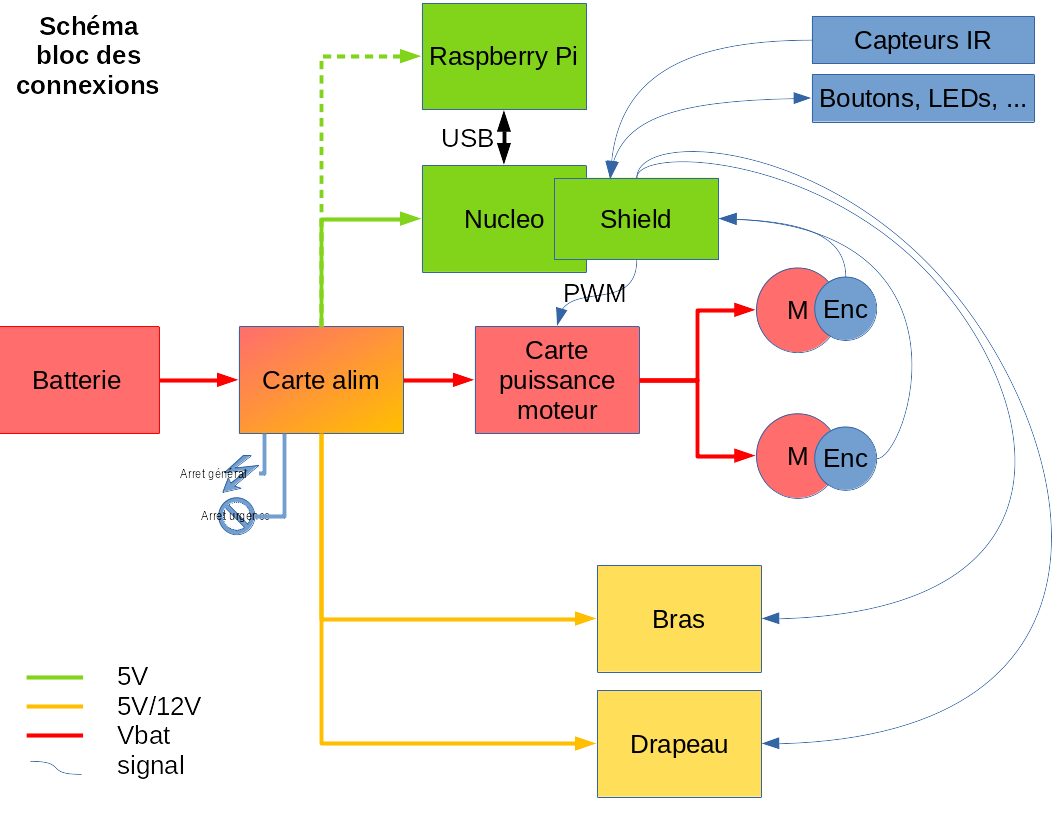
\includegraphics[scale=0.4]{schema_bloc_connexions.png}
  \caption{Schéma de principe de l'alimentation}
\end{figure}

\paragraph*{Point Puissance.}
Nous réutilisons les moteurs des 2A, le groupe travaillant dessus commence à
travailler.

\paragraph*{Point actionneur.}
Cnf tenaq pubfr à qver

\newpage
\section*{Jeudi 5 Décembre}
C'est bientôt Noël
\paragraph*{Point Table.}
Tous les éléments sont découpés et assemblés. Les manches à air sont montés et
la boussole est en cours de montage. Il restera les balises et au un écueil.

\paragraph*{Point Mécanique.}
L'étage du bas est modélisé, en attente de découpage. Nans a commandé les
profilés, la base pourra donc être montée sous peu.

\paragraph*{Point Phare.}
Le projet de l'ancien phare est correctement entéré. Marius est parti sur un
nouveau phare avec une base de bras robot comme ci contre.
\begin{figure}[H]
  \center
  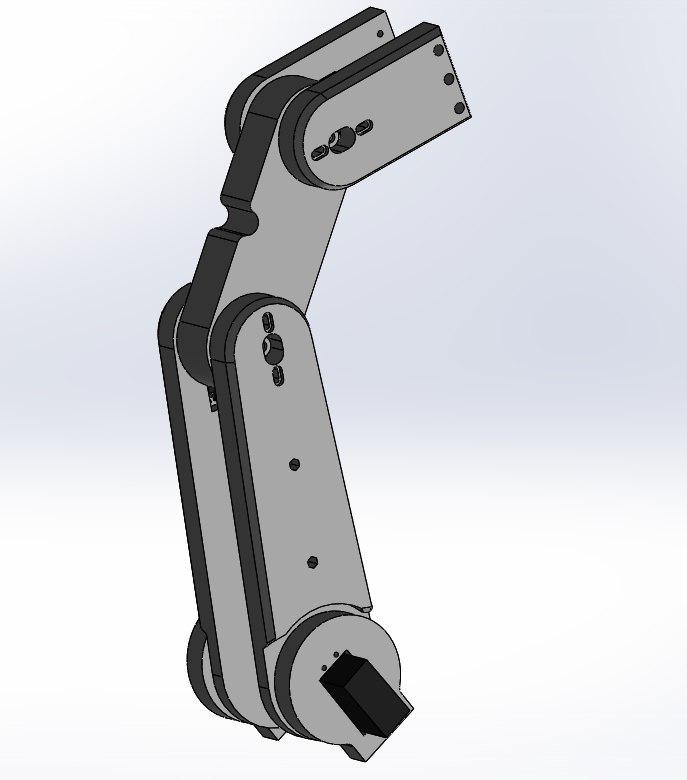
\includegraphics[scale=0.3]{phare.jpg}
  \caption{Version 2 du phare}
\end{figure}

\paragraph*{Point Asservissement + Info.}
Sébastien et Emile se battent avec le C++, Emile travaille sur les informations
renvoyées par les encodeurs pendant que Sébastien réflechit aux structures
qui permettrons au robot de correctement se déplacer.

\paragraph*{Point Alimentation.}
La carte d'alimentation avance bien, le travail de conception est en cours le
schéma de la carte d'alimentation sera disponible la semaine prochaine.

\paragraph*{Point Puissance.}
Y'vqér rfg q'nggraqer Znegva , cnepr dh'vy nvzr znatre qrf enqvngrhef nanybtvdhrf

\paragraph*{Point Actionneur.}
Les actionneurs sont au point morts pour l'instant, ce n'est pas l'urgence.

\newpage
\section*{Jeudi 12 Décembre}
Y avait du monde
\paragraph{Point Mécanique.}
Le dossier github de le méca a été crée et actualisé, on attend les profilés.
\paragraph{Point Phare.}
Le phare est en cours d'impression cela va prendre plusieurs jours.
\paragraph{Point Puissance.}
Le code de contrôle des moteurs a été conçu par Emile. L'utilisation de deux
ponts en H (LMD18200) est actée. Les moteurs fonctionnent en 16V ils seront donc
directement mis sur la batterie. La communication entre Ptit Lu et Martin est
faite.
\paragraph{Point Asservissement.}
L'idée est plutot d'attendre Clément et son expérience. Emile a testé les deux
moteurs ils sont bons, les encodeurs sont en cours de test. Grâce à Matthieu,
Emile arrive à utiliser la Nucléo. Le code a été commencé, Liam réfléchit à la
théorie de manière assez poussée.
\paragraph{Point Informatique.}
Grâce à OpenClassRoom Sébastien sait faire du C++ (enfin en théorie).
L'algorithme de recherche de chemin est semi-implémenté grâce au projet ours.
L'interface du robot n'a pas commencé.
\paragraph{Point Alimentation.}
Ptit Lu a dit : ``Mangez 5 fruits et légumes, c'est bon pour la santé.''
Le rootage de la carte doit débuter ce soir et on met pas de radiateur pour
faire en sorte que le robot ait plus de chance de bruler. Le récapitulatif du
schéma électrique est disponible dans les descriptions.


\newpage
\section*{Jeudi 16 Janvier}
\paragraph{Point Mécanique.}
La base du robot a été découpé ce jeudi. Le montage devrait avoir lieu dans la semaine
\paragraph{Point Phare.}
Le phare est en cours d'impression cela va prendre plusieurs jours. Mais il est
stylé de ouf.
\paragraph{Point Puissance.}
Le design est fait à priori.
\paragraph{Point Asservissement.}
Retour de Clément ! Il a fabriqué un banc de test et commencer à tester quelques
codes. Alban a dispensé une petite formation sur mbed pour les aider.
\paragraph{Point Informatique.}
Discussions sur le protocole de communication entre la Raspberry Pi et la
Nucléo. Utilisation d'une liaison série (via USB sûrement).
Présentation des avancements de la stratégie et schéma récapitulatif de cette dernière :
\begin{center}
  \begin{tikzpicture}
  \tikzstyle{lien}=[->,>=stealth,rounded corners=20pt,thick]
\tikzset{individu/.style={draw,thick,fill=#1!25},
individu/.default={white}, rounded corners=4pt}
\node[individu=violet] (A) at (0,0){\textsc{Main}};
\draw(1,0) node[right]{Envoie les ordres};
\draw(1,-0.5) node[right]{au fur et à mesure};
\node[individu=blue!50!black] (B) at (0,2){Navigation};
\draw(1,2) node[right]{$\leftarrow$ Calcul d'un};
\draw(1,1.5) node[right]{\; \; chemin précis};
\draw(-1,2) node[left]{Transformation en $\leftarrow$};
\draw(-1,1.5) node[left]{chemin global \;\;\;};

\node[individu=blue] (C) at (3,4){World};
\draw (4,4) node[right]{Renseigne position};
\draw (4,3.5) node[right]{obstacles};
\node[individu=green] (D) at (-3,4){Asservissement};
\draw (-4.5,4) node[left]{Permet d'envoyer};
\draw (-4.5,3.5) node[left]{requete déplacement};
\node[individu=blue!50!black] (E) at (-4,0){Evitemment};
\draw (-5,0) node[left]{Court circuite};
\draw (-5,-0.5) node[left]{le main};
\node[individu=green] (F) at (-3,-2){Détection};
\draw (-3,-2.5) node[below]{Renseigne GP2};
\node[individu=green] (G) at (3,-2){Actionneur};
\node[individu] (H) at (3,-4){Affichage};

\draw[lien] (A) -- (B);
\draw[lien] (A) -- (F);
\draw[lien] (A) -- (G);
\draw[lien] (F) -- (A);
\draw[lien] (B) -- (D);
\draw[lien] (C) -- (B);
\draw[lien] (E) -- (B);
\draw[lien] (F) -- (E);


  \end{tikzpicture}
\end{center}

\paragraph{Point Alimentation.}
La 3ème tentative de fabrication de la carte d'alimentation a réussie (L'auteur
de ce rapport en a quand même raté deux :)) ! Perçage fini et soudures finies jeudi soir.

\newpage
\section*{Jeudi 23 Janvier}
(C'est mon anniversaire quand je tape se rapport, vous vous en foutez mais bon
:'), en plus vous comprennez pas qui est l'auteur, une fois Ptit Lu, une fois
moi, on est perdu)
\paragraph{Point Mécanique.} La découpe laser est cassée, Erwann devrait continuer la modélisation des étages
\paragraph{Point Alimentation.} La carte est finie, il faut tester la carte et
surtout penser aux cables , la gestion des cables devrait être gérée par Julien.
\paragraph{Point Puissance.} Martin n'a plus qu'à les imprimer (peut être aidé
par Julien) il faut vérifier l'empreinte des composants.
\paragraph{Point asservissement.} Liam a commencé le codage et la création des
classes, on a plutot tapé sur le haut niveau, il manque le traitement des
données par Clément. Emile a crée une conversation messenger (preuve de son
utilité moindre)
\paragraph{Point protocole de com.} (pourquoi c'est pas toi qui tape ce rapport
?) Le protocole est TRES bien avancé, on peut envoyer et recevoir des données
mais ça beug un peu
\paragraph{Point actionneur.} Filipe a travaillé !! (il a fait un pignon on se
chauffe pas trop non plus)
\paragraph{Point phare.} (Il est beau !!) On a imprimé 6 pièces sur 7 , il faut
encore créer la carte d'alimentation
\paragraph{Point information.} Il y a eu un peu de changement dans le principe,
maintenant lors d'une requete de déplacement l'asserv peut renvoyer : ``ok'',
``timeout'' ou ``detection'' cela a permis de fusionner facilement la détection
et la navigation.
\paragraph{Point compteur.} On a compris qu'il fallait compter les points,
julien s'en occupe.

\newpage
\section*{Jeudi 6 Février}
C'est le première réunion en salle de réunion, c'était sympa
\paragraph{Point Mécanique.}
A cause de la panne de la découpe laser les profilés n'ont pas pu être installé.
On félicite Erwann pour le défaut de conception sur les manches à Air :).
Plusieurs objectifs ont été fixé. Tout d'abbord Erwann devrait concevoir les
supports de GP2. Il commence aussi à réflechir à la méthode de construction de
la balise.
\paragraph{Point Alimentation.} Le cas général fonctionne très bien. Il faut
encore tester les cas critiques et commencer à les installer sur le robot.
\paragraph{Point Puissance.} Martin et Filipe travaillent désormais ensemble.
Ils se sont fixés deux semaines pour sortir une première version des cartes.
\paragraph{Point Shield.} (Oui c'est un nouveau point) Yohann à réalisé une
bonne partie de la conception, maintenant il faut qu'il récupère les
informations de tout le monde pour être sur de réaliser un shield précis. La
quête des informations commence.
\paragraph{Point Asservissement.} Il a passé 3 heures à installer MatLab,
malgrès sa modestie l'asservissement avance très bien. Le robot arrive à être
commandé (sans faire n'importe quoi), Matthieu l'a aidé pour faire une méthode
de caractérisation des moteurs. Cela prend du temps mais il avance très bien.
\paragraph{Point Stratégie.} Nous avons fait le lien entre la stratégie et le
protocole de Communication, actuellement lorsque la stratégie envoie une requête
à la nucléo, la requête est très bien envoyée et le retour est pour l'instant générique.
\paragraph{Point Nucléo.} Il faut réalisrr le cahier des charges pour Liam, il devra
gérer les GP2 (activation / desactivation, gérer la récupération des informations
), gérer les contacteurs et les actionneurs.
\paragraph{Point Phare.} IL EST BEAU !!! Il manque une pièce (le haut du phare),
il reste à faire le circuit imprimé et la communication avec le robot (433MHz).
\paragraph{Point Compteur.} Julien connait la datasheet par coeur, et le schéma
a été commencé sur Kicad.
\paragraph{Global.} L'organisation physique du robot a été pensé.

\newpage
\section*{Jeudi 13 Février}
\paragraph{Point Mécanique.} La découpe laser est réparée !! Le porte batterie
est modélisé et en cours d'impression. Les profilés vont pouvoir être installé
sous peu et les supports GP2 ne sont pas commencés. \\

\paragraph{Point Alimentation.} ``NON''.

\paragraph{Point Puissance.} Conception commencée.

\paragraph{Point Shield.} Il a commencé la conception mais il attend que l'on soit sur
de tous les pins etc.

\paragraph{Point Asservissement.} Clément a pratiqué Matlab et il a trouvé les
équations il faut encore faire les réglages du correcteur

\paragraph{Point Stratégie.} Il faut encore changer quelques trucs (comme la
prise en compte de la distance pour les obstacles)

\paragraph{Point Nucléo.} La réunion avec Liam a été effectuée, le travail reste
à faire

\paragraph{Point Phare.} Une solution pour l'éclairage a été trouvé, avec une
led 1W et un système de miroir comme un phare réel.

\newpage
\section*{Jeudi 20 Février}
Pas de réunion : finir dossier Cdiscount

\newpage
\end{spacing}
\end{document}
